% Options for packages loaded elsewhere
\PassOptionsToPackage{unicode}{hyperref}
\PassOptionsToPackage{hyphens}{url}
\PassOptionsToPackage{dvipsnames,svgnames,x11names}{xcolor}
%
\documentclass[
  letterpaper,
  DIV=11,
  numbers=noendperiod]{scrartcl}

\usepackage{amsmath,amssymb}
\usepackage{setspace}
\usepackage{iftex}
\ifPDFTeX
  \usepackage[T1]{fontenc}
  \usepackage[utf8]{inputenc}
  \usepackage{textcomp} % provide euro and other symbols
\else % if luatex or xetex
  \usepackage{unicode-math}
  \defaultfontfeatures{Scale=MatchLowercase}
  \defaultfontfeatures[\rmfamily]{Ligatures=TeX,Scale=1}
\fi
\usepackage{lmodern}
\ifPDFTeX\else  
    % xetex/luatex font selection
\fi
% Use upquote if available, for straight quotes in verbatim environments
\IfFileExists{upquote.sty}{\usepackage{upquote}}{}
\IfFileExists{microtype.sty}{% use microtype if available
  \usepackage[]{microtype}
  \UseMicrotypeSet[protrusion]{basicmath} % disable protrusion for tt fonts
}{}
\usepackage{xcolor}
\setlength{\emergencystretch}{3em} % prevent overfull lines
\setcounter{secnumdepth}{5}
% Make \paragraph and \subparagraph free-standing
\makeatletter
\ifx\paragraph\undefined\else
  \let\oldparagraph\paragraph
  \renewcommand{\paragraph}{
    \@ifstar
      \xxxParagraphStar
      \xxxParagraphNoStar
  }
  \newcommand{\xxxParagraphStar}[1]{\oldparagraph*{#1}\mbox{}}
  \newcommand{\xxxParagraphNoStar}[1]{\oldparagraph{#1}\mbox{}}
\fi
\ifx\subparagraph\undefined\else
  \let\oldsubparagraph\subparagraph
  \renewcommand{\subparagraph}{
    \@ifstar
      \xxxSubParagraphStar
      \xxxSubParagraphNoStar
  }
  \newcommand{\xxxSubParagraphStar}[1]{\oldsubparagraph*{#1}\mbox{}}
  \newcommand{\xxxSubParagraphNoStar}[1]{\oldsubparagraph{#1}\mbox{}}
\fi
\makeatother


\providecommand{\tightlist}{%
  \setlength{\itemsep}{0pt}\setlength{\parskip}{0pt}}\usepackage{longtable,booktabs,array}
\usepackage{calc} % for calculating minipage widths
% Correct order of tables after \paragraph or \subparagraph
\usepackage{etoolbox}
\makeatletter
\patchcmd\longtable{\par}{\if@noskipsec\mbox{}\fi\par}{}{}
\makeatother
% Allow footnotes in longtable head/foot
\IfFileExists{footnotehyper.sty}{\usepackage{footnotehyper}}{\usepackage{footnote}}
\makesavenoteenv{longtable}
\usepackage{graphicx}
\makeatletter
\def\maxwidth{\ifdim\Gin@nat@width>\linewidth\linewidth\else\Gin@nat@width\fi}
\def\maxheight{\ifdim\Gin@nat@height>\textheight\textheight\else\Gin@nat@height\fi}
\makeatother
% Scale images if necessary, so that they will not overflow the page
% margins by default, and it is still possible to overwrite the defaults
% using explicit options in \includegraphics[width, height, ...]{}
\setkeys{Gin}{width=\maxwidth,height=\maxheight,keepaspectratio}
% Set default figure placement to htbp
\makeatletter
\def\fps@figure{htbp}
\makeatother

\usepackage{fontspec}
\usepackage{multirow}
\usepackage{multicol}
\usepackage{colortbl}
\usepackage{hhline}
\newlength\Oldarrayrulewidth
\newlength\Oldtabcolsep
\usepackage{longtable}
\usepackage{array}
\usepackage{hyperref}
\usepackage{float}
\usepackage{wrapfig}
% \usepackage{hyperref}
% \hypersetup{
%     colorlinks,
%     linkcolor={blue!100!black},
%     citecolor={blue!100!black},
%     urlcolor={blue!100!black}
% }
% \usepackage{apacite}
% \usepackage[round]{natbib} 
% \usepackage{graphicx}
% \usepackage{float}
% \usepackage{caption}
% \usepackage[toc,page]{appendix}
% \usepackage{booktabs,caption}
% \usepackage[flushleft]{threeparttable}
% \usepackage{tabularx}
\usepackage{sfmath}
\usepackage{fontspec}
\usepackage[utf8]{inputenc}
\usepackage{siunitx}
\usepackage{amsfonts}
\usepackage{amsmath}
% \usepackage{xcolor}
% \usepackage{scrextend}
% \deffootnote[2em]{2em}{1em}{\textsuperscript{\thefootnotemark}\,}
% \newcolumntype{Y}{>{\centering\arraybackslash}X}
% \usepackage[a4paper]{geometry}
% \usepackage{caption}
% \usepackage[bottom,flushmargin,hang,multiple]{footmisc}
% \usepackage{pdflscape}
% \usepackage[paper=portrait,pagesize]{typearea}
% \usepackage{rotating}
% \usepackage{fullpage}
% \usepackage{tabu}
\usepackage{lscape}
\newcommand{\blandscape}{\begin{landscape}}
\newcommand{\elandscape}{\end{landscape}}
\usepackage{rotating}
\newcommand{\bsideways}{\begin{sidewaystable}[htbp]}
\newcommand{\esideways}{\end{sidewaystable}}
\KOMAoption{captions}{tableheading}
\makeatletter
\@ifpackageloaded{caption}{}{\usepackage{caption}}
\AtBeginDocument{%
\ifdefined\contentsname
  \renewcommand*\contentsname{Table of contents}
\else
  \newcommand\contentsname{Table of contents}
\fi
\ifdefined\listfigurename
  \renewcommand*\listfigurename{List of Figures}
\else
  \newcommand\listfigurename{List of Figures}
\fi
\ifdefined\listtablename
  \renewcommand*\listtablename{List of Tables}
\else
  \newcommand\listtablename{List of Tables}
\fi
\ifdefined\figurename
  \renewcommand*\figurename{Figure}
\else
  \newcommand\figurename{Figure}
\fi
\ifdefined\tablename
  \renewcommand*\tablename{Table}
\else
  \newcommand\tablename{Table}
\fi
}
\@ifpackageloaded{float}{}{\usepackage{float}}
\floatstyle{ruled}
\@ifundefined{c@chapter}{\newfloat{codelisting}{h}{lop}}{\newfloat{codelisting}{h}{lop}[chapter]}
\floatname{codelisting}{Listing}
\newcommand*\listoflistings{\listof{codelisting}{List of Listings}}
\makeatother
\makeatletter
\makeatother
\makeatletter
\@ifpackageloaded{caption}{}{\usepackage{caption}}
\@ifpackageloaded{subcaption}{}{\usepackage{subcaption}}
\makeatother

\ifLuaTeX
  \usepackage{selnolig}  % disable illegal ligatures
\fi
\usepackage[round]{natbib}
\bibliographystyle{apalike}
\usepackage{bookmark}

\IfFileExists{xurl.sty}{\usepackage{xurl}}{} % add URL line breaks if available
\urlstyle{same} % disable monospaced font for URLs
\hypersetup{
  colorlinks=true,
  linkcolor={blue!100!black},
  filecolor={Maroon},
  citecolor={blue!100!black},
  urlcolor={blue!100!black},
  pdfcreator={LaTeX via pandoc}}


\author{}
\date{}

\begin{document}

\title{Inflation in times of global warming}


\author {Xolani Sibande\footnote{Economic Research Department, South African Reserve Bank; Email: xolani.sibande@resbank.co.za.} \and
Serena Merrino \footnote{Economic Research Department, South African Reserve Bank and University College London, School of Slavonic and East European Studies, United Kingdom; Email: serena.merrino@resbank.co.za}}


\date{\today}
\maketitle

\begin{abstract}
ipsum

\end{abstract}

\noindent\textbf{Keywords}: Climate impacts, Input-output supply chain interlinkages, Pro-
duction network, Spillovers, Weather shocks, Monetary Policy
\textbf{JEL Codes}:E23, E32, E52, L14, O11, Q54, R15,
\newpage


\setstretch{1.5}
\section{Introduction}\label{introduction}

The post-pandemic surge of inflation to a four-decade high in many
advanced and emerging markets has renewed interest in the drivers of
aggregate inflation and prompted questions on the optimal response of
the monetary authorities to deviations from target (ref: Chris Giles,
FT). While the consensus is strong with respect to the need for curbing
excess demand-pull inflation by means of monetary tightening, adverse
supply shocks that push prices up and output down create difficult
policy trade-offs \citep{klomp2020}. A key tenet of modern monetary
policymaking under flexible average inflation-targeting regimes is
indeed to ``look through'' transitory trade-off inducing supply shocks,
especially if originated in specific markets, unless their persistence
threatens the stability of expectations and inflation to become
entrenched (\ldots). On these lines, although the recent inflationary
episode was supposedly driven by a series of idiosyncratic developments
- namely, supply-chain bottlenecks, changes in relative prices, and
Russia's invasion of Ukraine, possibly exacerbated by firms' excessive
market power \citep{stiglitz2023} - central banks have responded by
sustaining high interest rates purportedly to slay aggregate demand. In
the latest BIS annual report, such forceful global tightening action is
celebrated for it sent ``a strong signal to markets, firms and workers
that the central bank would do what it took to restore price stability''
(BIS 2024, p.~\ldots). As a result, ``inflation is now again returning
to the price stability region while economic activity and labour markets
have proved resilient'' (idib., p.~\ldots). In academic circles,
however, the firm adoption of a contractionary stance is generally seen
as a blunt and unnecessarily costly revival of the monetarist doctrine,
which overshadows alternative instruments of price stabilisation
\citep[see, for example,][]{stiglitz2023, weber2023}. Correctly
identifying the origins of inflation (along with producing reliable
forecasts and indicators of future expectations) is key to tailoring an
appropriate policy response.

As these shocks wane and inflation comes down, the two narratives on the
origins of inflation remain appropriate in the context of another,
increasingly concerning, source of future uncertainty. Climate change is
an accelerating process that is expected to increase the frequency and
intensity of both acute physical hazards (i.e., droughts, floods,
wildfires, heatwaves, etc.) and chronic deviations of meteorological
variables from historical means (i.e., rising averages in temperature
and precipitation) (IPCC 2021). The physical risks deriving from these
phenomena influence agents' preferences and endowments with immediate
implications for the price stability mandate of central banks around the
world through a variety of supply- and demand-side channels (we review
them in Section 2). In contrast to the longer-run changes in climatic
trends which influence the optimal monetary policy and r-star
\citep{mukherjee2021}, extreme climatic events ``are largely
unpredictable and thereby bear resemblance to other shocks that unfold
over the business cycle and to which monetary policymakers tend to
adjust monetary policy'' (NGFS, 2024, p.~7). Either way, climate change
is flaring up the debate over whether policymakers should respond to
climate-induced inflationary pressures in the same old way --- by
vigorous monetary tightening.

This paper aims to contribute to this discussion by providing new
evidence on the effect of acute climatic events on inflation employing a
global panel dataset of monthly country-sector inflation from 2000 to
2023. We add to existing studies in several ways. First, we zoom in on
12 Consumer Price sub-indexes and 6 PPI sub-categories to disentangle
the idiosyncratic nature (sectoral, cost-push vs demand-pull) of the
impact of acute physical hazards (i.e., deviations in rainfall,
temperature, and dryness).\footnote{We use the COICOP price
  classification, that is a United Nations international reference
  framework for grouping household consumption expenditures on goods and
  services within homogeneous categories (UNSD, 1991).} Secondly, we
acknowledge the importance of the production network in the propagation
of price spillovers and aggregate inflation dynamics. While there is
broad agreement that the degree to which sectoral prices respond to
shocks is determined by the input-output structure of the economy, there
is no evidence for the transmission mechanisms responsible for the
inflationary effects of climate change. To fill this gap, we build upon
the literature on sectoral propagation of shocks (\ldots), recently
applied to assess the impact of weather shocks and sectoral productivity
by \citet{zappala2024}, to develop an input-output framework that
factors in the indirect price spillover effects of weather shocks. In
addition, we follow current developments in the scholarship on inflation
determinants by accounting for possible moderating and mediating
factors, such as the role of sectoral competition in the price setting
mechanism \citep{weber2023} and the monetary policy stance.

While the empirical analysis is global in essence, the econometric model
will be also specified as a country-specific regression to examine the
experience of a single economy: we choose South Africa. Southern Africa
is a climate-sensitive region that is already experiencing significant
deviations of rainfall and temperatures from long-term averages as well
as severe droughts and floods (World Bank Climate Portal 2024), with
implications for water availability and food security. From a
socio-economic perspective, however, South Africa is the strongest
country in the region, exhibiting a solid infrastructure and a
well-diversified and emerging open economy fully integrated to global
supply chains. Moreover, what makes South Africa a good case study is
its high levels of market concentration and product regulation to
validate the existence of profit-led inflation.

Notably, our sectoral approach does not downplay the macroeconomic
relevance of climate risk. On the contrary, shedding light on how
climate change affects specific segments of the economy and spills over
to other sectors is key to understand macroeconomic processes, such as
the underlying nature of aggregate inflation, and to envisage tailored
policy responses. Relative price changes are also fundamental to the
analysis of welfare costs, as heterogeneous households face different
inflation rates depending on their income, wealth, and composition of
their consumption basket (\ldots). Thus, despite their merits, not only
aggregate indexes can potentially smoothen out the variance from several
inflation components, but they also conceal the true inflation costs
that different consumers within the same country are susceptible to.
Similarly, we are aware that a possible limitation of our study derives
from the risk country-level data veil some of the localised effects of
changing weather conditions but, even so, the sectoral dimension should
be sufficiently sensible.\footnote{If, for example, the shock hits only
  one of the nine provinces of South Africa, and raises food prices
  there, local food inflation will show up in the national food price
  index if the affected province's food sector has a large enough share
  or if it travels to other regions through intra-national trade. If,
  instead, the local sector share is negligible (price-taker), local
  inflation is likely to disappear.}

Finally, the present analysis is limited to `climateflation', first
defined by \citet{schnabel2022} to conceptualise the ways in which
physical risks caused by climate change put upside pressure on prices.
In particular, we focus here on a wide range of acute severe climatic
events. Other aspects are important in determining the relation between
weather and price movements, such as the impact of chronic rises in
temperature averages, climate adaptation and mitigation policies, but
these are beyond the scope of this paper.

\section{Climateflation: A literature
review}\label{climateflation-a-literature-review}

The past few years have witnessed growing efforts of the research
community towards the empirical assessment of the socio-economic effects
of climate change. Although the causal relation between climate and
prices remains understudied, existing empirical works find that the
response of aggregate inflation to climate change is varied.
\citet{parker2018} and \citet{cevik2023} highlight the importance of the
type of climate-induced natural disaster, the country's level of
development and fiscal space in determining the direction and size of
the inflation effect whereas, focusing at the effects of temperature
deviations, \citet{mukherjee2021} and \citet{kotz2024} document rising
and persistent inflation, especially in lower-income countries.

Along with the diversity of climate-induced shocks, also the channels of
price transmission are multiple and convoluted: for example, shocks can
hit the supply or demand-side of the economy, directly or indirectly,
they can be physical or non-physical, sudden or progressive, and they
can travel upstream or downstream the economic system. This mix of
possibilities means ``no two physical hazard events have the same
macroeconomic effects`` (NGFS 2024, p.~9) and that different weather
shocks will likely hit different segments of the economy, often
unevenly, causing volatility both in nominal and relative prices
\citep{buelens2024}. We attempt to conceptualise the mechanisms behind
climateflation here. Climate-induced supply shocks. On the supply side,
the climate influences some of the characteristics and effective
availability of productive factors -- such as impoverishment of natural
resources, a more rapid depreciation of capital endowments, or reduction
in labour - and total factor productivity, that encapsulates the role of
technology, financing conditions, infrastructure, supply chain
disruptions, etc. (NGFS, 2024).

Sectors characterised by an inherent exposure to weather-based risk are
particularly sensitive to the direct effect of local weather shocks. In
farming, for example, changes in weather conditions impact negatively on
agricultural productivity through workers' heat stress
\citep{delima2021}, environmental degradation affecting crops and animal
breeding \citep{liang2017} or increased use of pesticides and overall
production costs (Savage 2024). Many authors have focused on the
climate-food prices relationship. \citet{faccia2021} find that upward
temperature anomalies have an immediate impact on food prices;
\citet{kotz2024} observe that the effects of global warming are
strongest in the food component of inflation; Roberts and Schlenker
(2013) find that crop yields are humped-shaped, with higher temperatures
increasing yields up until a threshold, before having increasingly
negative effects. Finally, according to Parker (2016) storms and floods
lead to a short-lived but upward effect on food price inflation.

As the climate warms, disruptions in the water cycle are likely to hit
water-intensive sectors, including not only agriculture but also
electricity, manufacturing, and waterway transport \citep{buelens2024}.
Also, the higher demand for energy for cooling and warming, as climate
becomes extreme, will increase its price as well as the chances of power
disruptions \citep{mukherjee2021}. An additional direct impact is
observed in the NGFS (2023)'s report and relates to damages inflicted on
ecosystems resulting in the loss of services, such as touristic, from
these systems.

Direct adverse effects on productivity can also emerge due to reduced
number of working hours or to presenteeism, due to heat stress and
impaired health conditions among others (Graff Zivin et al.~2018, ILO
2019, Nath 2020, Pinna Pintor et al.~2024). Lower labour productivity
can result in non-agricultural sectors too, particularly in presence of
outdoor work (e.g.~construction, tourism), but also in indoor settings
(e.g.~factories or offices) (ILO 2019). Acevedo et al.~(2020) documents
that higher temperatures significantly lower labour productivity in
heat-exposed sectors but they have no significant effect in non-heat
exposed industries, including in hot climate countries. Some authors
additionally highlight the presence of seasonally heterogenous
pressures, such that increases in hotter months and regions reduce the
growth rate of labour productivity and GDP \citep{colacito2019} and
possibly cause larger inflationary impacts \citep{kotz2024}, while
warmer winter temperatures are associated with lower energy prices.
Reduction in total factor productivity \citep{letta2019}, or damages and
faster depreciation of capital assets \citep{bakkensen2018} have also
been documented.

In all these cases, higher costs of production in the affected sectors
are transmitted downstream as higher end-user and wholesale prices.
There is a growing body of literature that highlights the role of
economic networks, where shocks that hit sectors or firms propagate
through input-output linkages leading to large aggregate
effects.\footnote{See Long and Plosser (1983); Shea (2002); Gabaix
  (2011); Acemoglu et al.~(2012); Di Giovanni et al.~(2014); Acemoglu et
  al.~(2016); Magerman et al.~(2016); Grassi (2017); Huneeus (2018); Lim
  (2018); Baqaee and Farhi (2019).} \citet{acemoglu2012} show that in
the presence of intersectoral input--output linkages, microeconomic
idiosyncratic shocks may lead to ``cascade effects'' whereby
productivity shocks to a sector located in the early stages of the
supply chain propagate not only to its immediate downstream customers,
but also to the rest of the economy. \citet{dewinne2018} find that
adverse weather impacts on agricultural production and food commodity
prices can depress economic activity worldwide, including in high-income
countries. \citet{zappala2024} uses the input-output framework to
examine the productivity shock transmission across sectors and shows
that, although agriculture is harmed the most and earlier, downstream
sectors -- even if foreign - suffer from substantial and persistent
losses as a result of network effects.

The price transmission mechanism occurs along similar lines: upstream
price changes -- such as in agriculture and electricity - percolate
downstream: ``The producer price of an industry depends on both the
prices/volume of its input suppliers and sector-specific productivity
shocks. (\ldots) Price shocks in the machinery industry affects the
price of motor vehicles because of the production network coefficient.''
(Bilgin 2022, p.~14) Moreover, the mechanism is asymmetric because
downstream prices adjust downward more rapidly than they would do
upward, and at a lower passthrough rate. In contrast to production, in
the inflation diffusion network the central nodes are the upstream
industries that by supplying intermediate inputs to others lead to cost
pass-through. The latter will be stronger if it originates in
``salient'' commodities (e.g.~oil, food). In the euro area,
\citet{peersman2022} estimates that shifts in international food prices
between 1961 and 2016, caused by harvest shocks, explain 30\% of
euro-area inflation volatility. Also, \citet{ciccarelli2023} document
that temperature increases raise EU inflation in food and services,
possibly due to higher sensitivity of services, such as health and
tourism, to food or weather. Di Giovanni et al.~(2022) reveal that Euro
Area inflation amplified through production networks after the pandemic.
Depending on the elasticity of substitution between inputs, the
reallocation of expenditure can mitigate the ripple effect of the
production cost shock. If however demand remains stable, input price
increases are otherwise passed on to consumers as cost-push
inflation.\footnote{If demand is perfectly elastic, producers will be
  forced to fully absorb the shock. On the contrary, if demand is
  perfectly inelastic, consumers will be forced to buy the good whatever
  the price is.} \citet{weber2023} posit that in advanced economies
firms with big market power have contributed to recent inflation by
amplifying the initial supply disruptions in essential sectors, such as
food and energy.

Overall, relative price adjustments that pass through to broad-based
inflation (``first-round effects'') can generate durable implications
for medium-run inflation, expectations, wages (``second-round
effects''), and the conduct of monetary policy {[}\citet{reis2010}; BIS
2022{]}. At the same time, as noted by NGFS (2021), more frequent
climate shocks will make it more difficult to disentangle permanent from
transitory shocks. Moreover, food inflation is often perceived by
households as a signal of future inflation, which will be then embedded
in their expectation formation. All these factors induce central banks
to intervene. According to \citet{mukherjee2021}, in developing
countries, price effects persist several years after the initial shock.
The reasons can be multiple: first, poor integration into global markets
implies weak import substitution effects (i.e., a failed local harvest
is not easily substituted with food imports) and, secondly, food prices
in developing countries depend on weather more than in advanced
countries where the relative contribution of wages, physical capital,
energy, and transport costs is substantially higher.

Climate-induced demand shocks. Beyond driving cost-push inflation up,
the climate can also shift household preferences and human needs
(e.g.~cooling or warming) and by extension demand patterns. For example,
depressed economic activity (i.e., declining income, wealth, and
confidence) might cause falling prices for non-tradable sectors
\citep{kamber2013}. Particularly in developing countries where food
constitutes the largest share of the consumer basket, higher food prices
reduce the money available for other items, stifling broader consumer
spending. In a cross-country analysis of 48 advanced and emerging
economies, \citet{faccia2021} find that upward temperature anomalies
have a swift upward effect which turns insignificant or even negative in
the medium term, possibly due to lower demand. Distinguishing by type
and intensity of climate shocks, \citet{Kabundi2022} find that, while
droughts tend to push inflation up because of rising food prices, floods
curb demand and so inflation. In the aftermath of a weather shock,
consumption patterns may adapt in ways that prompt relative price
fluctuations among sectors, such as from hospitality and travel to
technology. Explained in Figure~\ref{fig-flowchart}.

In contrast to the spillover effects of supply-side shocks, demand
shocks do not give rise to price transmission from customers to
suppliers despite the presence of sectoral interlinkages: for example,
if as a result of a weather shock consumers' demand for hospitality
falls, this will likely affect the price of the focal sector (i.e.,
hospitality sector) without altering the price of its suppliers
(i.e.~food or construction industry).\footnote{A few authors study
  demand shocks' transmission across sectoral production and highlight
  specific conditions whereby upstream propagation may arise (Acemoglu
  et al.~2012, Arata and Miyakawa 2022).}

Furthermore, Ferrante et al (2023) note that the post-pandemic
inflationary effects of the demand reallocation from services to goods
were amplified by the sectoral heterogeneity in price rigidity:
industries that produce goods have more flexible prices than those that
produce services and so service-producing sectors reduce production
swiftly, with only modest declines in prices. Thus, another important
question to understand the origins of aggregate inflation is whether
climate change spurs demand in sectors with relatively more flexible
prices than shrinking sectors.

\begin{figure}[h]

\centering{

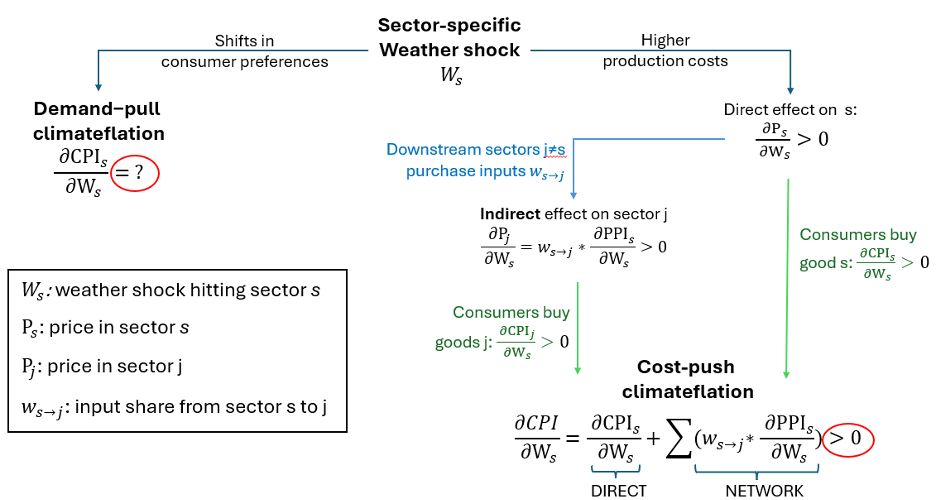
\includegraphics[width=3.12in,height=\textheight]{flow_chart.png}

}

\caption{\label{fig-flowchart}Flow chart of price propagation from
weather shocks}

\end{figure}%

In summary, a weather shock translates into idiosyncratic inflation via
three channels: (i) on the demand-side, the price effect is ambiguous
and depends on the sector-specific demand response to the weather shock;
on the supply-side, (ii) a sector-specific weather shock changes the
price in that sector directly and, lastly, (iii) by affecting the price
of any other sector that supply inputs to the focal sector, it travels
downstream (network weather shock). The cross-sector sum of these
effects will result into aggregate inflation.

Given the complex interplay of upward and downward forces on prices, the
overall reaction of inflation to weather shocks depends on which
countervailing dynamic dominates \citep{parker2018}. Moreover, ``a
negligible or null effect of local weather shocks on a given sector may
be amplified or mitigated by weather shocks hitting other sectors with
strong commercial inter linkages'' \citep{zappala2024}. Climate change
is therefore highly sectoral by nature.

\section{Data}\label{data}

\subsection{Prices}\label{prices}

We build a global dataset of monthly Consumer Price indexes and sectoral
sub-indexes sourced from Haver Analytics. We use non-seasonally adjusted
data due to better coverage and we remove seasonal effects. By matching
the 12 CPI categories which classify consumer expenditure to the
standard taxonomy of industrial sectors (UN 2008), we derive sectoral
retail prices -- see Table~\ref{tbl-cpi_matching}.\footnote{We exclude
  `Alcohol and Tobacco' prices as well as `Other' prices due to the
  impossibility of properly matching these products to a particular
  industrial sector.} Our sample covers 151 countries from January 1980
to December 2023; however, to make the panel more balanced, we restrict
the analysis to the period 2000-2023 (details on data availability per
country-sector are in Table A1 in the Appendix).

\newpage

\global\setlength{\Oldarrayrulewidth}{\arrayrulewidth}

\global\setlength{\Oldtabcolsep}{\tabcolsep}

\setlength{\tabcolsep}{2pt}

\renewcommand*{\arraystretch}{0.5}



\providecommand{\ascline}[3]{\noalign{\global\arrayrulewidth #1}\arrayrulecolor[HTML]{#2}\cline{#3}}

\begin{longtable}[l]{|p{0.94in}|p{1.69in}|p{2.91in}}

\caption{\label{tbl-cpi_matching}Matching price categories to industrial
sectors}

\tabularnewline

\ascline{1pt}{000000}{1-3}

\multicolumn{1}{!{\color[HTML]{FFFFFF}\vrule width 1pt}>{\raggedright}m{\dimexpr 0.94in+0\tabcolsep}}{\textcolor[HTML]{000000}{\fontsize{7}{7}\selectfont{\global\setmainfont{Arial}{No.}}}} & \multicolumn{1}{!{\color[HTML]{FFFFFF}\vrule width 1pt}>{\raggedright}m{\dimexpr 1.69in+0\tabcolsep}}{\textcolor[HTML]{000000}{\fontsize{7}{7}\selectfont{\global\setmainfont{Arial}{CPI\ category}}}} & \multicolumn{1}{!{\color[HTML]{FFFFFF}\vrule width 1pt}>{\raggedright}m{\dimexpr 2.91in+0\tabcolsep}!{\color[HTML]{FFFFFF}\vrule width 1pt}}{\textcolor[HTML]{000000}{\fontsize{7}{7}\selectfont{\global\setmainfont{Arial}{Industry\ Classification}}}} \\

\ascline{1pt}{000000}{1-3}\endfirsthead 

\ascline{1pt}{000000}{1-3}

\multicolumn{1}{!{\color[HTML]{FFFFFF}\vrule width 1pt}>{\raggedright}m{\dimexpr 0.94in+0\tabcolsep}}{\textcolor[HTML]{000000}{\fontsize{7}{7}\selectfont{\global\setmainfont{Arial}{No.}}}} & \multicolumn{1}{!{\color[HTML]{FFFFFF}\vrule width 1pt}>{\raggedright}m{\dimexpr 1.69in+0\tabcolsep}}{\textcolor[HTML]{000000}{\fontsize{7}{7}\selectfont{\global\setmainfont{Arial}{CPI\ category}}}} & \multicolumn{1}{!{\color[HTML]{FFFFFF}\vrule width 1pt}>{\raggedright}m{\dimexpr 2.91in+0\tabcolsep}!{\color[HTML]{FFFFFF}\vrule width 1pt}}{\textcolor[HTML]{000000}{\fontsize{7}{7}\selectfont{\global\setmainfont{Arial}{Industry\ Classification}}}} \\

\ascline{1pt}{000000}{1-3}\endhead



\multicolumn{1}{!{\color[HTML]{FFFFFF}\vrule width 1pt}>{\raggedright}m{\dimexpr 0.94in+0\tabcolsep}}{\textcolor[HTML]{000000}{\fontsize{7}{7}\selectfont{\global\setmainfont{Arial}{1}}}} & \multicolumn{1}{!{\color[HTML]{FFFFFF}\vrule width 1pt}>{\raggedright}m{\dimexpr 1.69in+0\tabcolsep}}{\textcolor[HTML]{000000}{\fontsize{7}{7}\selectfont{\global\setmainfont{Arial}{Headline}}}} & \multicolumn{1}{!{\color[HTML]{FFFFFF}\vrule width 1pt}>{\raggedright}m{\dimexpr 2.91in+0\tabcolsep}!{\color[HTML]{FFFFFF}\vrule width 1pt}}{\textcolor[HTML]{000000}{\fontsize{7}{7}\selectfont{\global\setmainfont{Arial}{All\ economic\ activities}}}} \\

\ascline{1pt}{FFFFFF}{1-3}



\multicolumn{1}{!{\color[HTML]{FFFFFF}\vrule width 1pt}>{\raggedright}m{\dimexpr 0.94in+0\tabcolsep}}{\textcolor[HTML]{000000}{\fontsize{7}{7}\selectfont{\global\setmainfont{Arial}{2}}}} & \multicolumn{1}{!{\color[HTML]{FFFFFF}\vrule width 1pt}>{\raggedright}m{\dimexpr 1.69in+0\tabcolsep}}{\textcolor[HTML]{000000}{\fontsize{7}{7}\selectfont{\global\setmainfont{Arial}{Energy}}}} & \multicolumn{1}{!{\color[HTML]{FFFFFF}\vrule width 1pt}>{\raggedright}m{\dimexpr 2.91in+0\tabcolsep}!{\color[HTML]{FFFFFF}\vrule width 1pt}}{\textcolor[HTML]{000000}{\fontsize{7}{7}\selectfont{\global\setmainfont{Arial}{Electricity,\ gas,\ steam\ and\ air\ conditioning\ supply}}}} \\

\ascline{1pt}{FFFFFF}{1-3}



\multicolumn{1}{!{\color[HTML]{FFFFFF}\vrule width 1pt}>{\raggedright}m{\dimexpr 0.94in+0\tabcolsep}}{\textcolor[HTML]{000000}{\fontsize{7}{7}\selectfont{\global\setmainfont{Arial}{3}}}} & \multicolumn{1}{!{\color[HTML]{FFFFFF}\vrule width 1pt}>{\raggedright}m{\dimexpr 1.69in+0\tabcolsep}}{\textcolor[HTML]{000000}{\fontsize{7}{7}\selectfont{\global\setmainfont{Arial}{Food\ and\ Beverages}}}} & \multicolumn{1}{!{\color[HTML]{FFFFFF}\vrule width 1pt}>{\raggedright}m{\dimexpr 2.91in+0\tabcolsep}!{\color[HTML]{FFFFFF}\vrule width 1pt}}{\textcolor[HTML]{000000}{\fontsize{7}{7}\selectfont{\global\setmainfont{Arial}{Agriculture,\ forestry\ and\ fishing}}}} \\

\ascline{1pt}{FFFFFF}{1-3}



\multicolumn{1}{!{\color[HTML]{FFFFFF}\vrule width 1pt}>{\raggedright}m{\dimexpr 0.94in+0\tabcolsep}}{\textcolor[HTML]{000000}{\fontsize{7}{7}\selectfont{\global\setmainfont{Arial}{4}}}} & \multicolumn{1}{!{\color[HTML]{FFFFFF}\vrule width 1pt}>{\raggedright}m{\dimexpr 1.69in+0\tabcolsep}}{\textcolor[HTML]{000000}{\fontsize{7}{7}\selectfont{\global\setmainfont{Arial}{Clothing}}}} & \multicolumn{1}{!{\color[HTML]{FFFFFF}\vrule width 1pt}>{\raggedright}m{\dimexpr 2.91in+0\tabcolsep}!{\color[HTML]{FFFFFF}\vrule width 1pt}}{\textcolor[HTML]{000000}{\fontsize{7}{7}\selectfont{\global\setmainfont{Arial}{Manufacturing}}}} \\

\ascline{1pt}{FFFFFF}{1-3}



\multicolumn{1}{!{\color[HTML]{FFFFFF}\vrule width 1pt}>{\raggedright}m{\dimexpr 0.94in+0\tabcolsep}}{\textcolor[HTML]{000000}{\fontsize{7}{7}\selectfont{\global\setmainfont{Arial}{5}}}} & \multicolumn{1}{!{\color[HTML]{FFFFFF}\vrule width 1pt}>{\raggedright}m{\dimexpr 1.69in+0\tabcolsep}}{\textcolor[HTML]{000000}{\fontsize{7}{7}\selectfont{\global\setmainfont{Arial}{Housing}}}} & \multicolumn{1}{!{\color[HTML]{FFFFFF}\vrule width 1pt}>{\raggedright}m{\dimexpr 2.91in+0\tabcolsep}!{\color[HTML]{FFFFFF}\vrule width 1pt}}{\textcolor[HTML]{000000}{\fontsize{7}{7}\selectfont{\global\setmainfont{Arial}{Real\ estate\ activities}}}} \\

\ascline{1pt}{FFFFFF}{1-3}



\multicolumn{1}{!{\color[HTML]{FFFFFF}\vrule width 1pt}>{\raggedright}m{\dimexpr 0.94in+0\tabcolsep}}{\textcolor[HTML]{000000}{\fontsize{7}{7}\selectfont{\global\setmainfont{Arial}{6}}}} & \multicolumn{1}{!{\color[HTML]{FFFFFF}\vrule width 1pt}>{\raggedright}m{\dimexpr 1.69in+0\tabcolsep}}{\textcolor[HTML]{000000}{\fontsize{7}{7}\selectfont{\global\setmainfont{Arial}{Household\ goods}}}} & \multicolumn{1}{!{\color[HTML]{FFFFFF}\vrule width 1pt}>{\raggedright}m{\dimexpr 2.91in+0\tabcolsep}!{\color[HTML]{FFFFFF}\vrule width 1pt}}{\textcolor[HTML]{000000}{\fontsize{7}{7}\selectfont{\global\setmainfont{Arial}{Manufacturing}}}} \\

\ascline{1pt}{FFFFFF}{1-3}



\multicolumn{1}{!{\color[HTML]{FFFFFF}\vrule width 1pt}>{\raggedright}m{\dimexpr 0.94in+0\tabcolsep}}{\textcolor[HTML]{000000}{\fontsize{7}{7}\selectfont{\global\setmainfont{Arial}{7}}}} & \multicolumn{1}{!{\color[HTML]{FFFFFF}\vrule width 1pt}>{\raggedright}m{\dimexpr 1.69in+0\tabcolsep}}{\textcolor[HTML]{000000}{\fontsize{7}{7}\selectfont{\global\setmainfont{Arial}{Transport}}}} & \multicolumn{1}{!{\color[HTML]{FFFFFF}\vrule width 1pt}>{\raggedright}m{\dimexpr 2.91in+0\tabcolsep}!{\color[HTML]{FFFFFF}\vrule width 1pt}}{\textcolor[HTML]{000000}{\fontsize{7}{7}\selectfont{\global\setmainfont{Arial}{Transportation\ and\ storage}}}} \\

\ascline{1pt}{FFFFFF}{1-3}



\multicolumn{1}{!{\color[HTML]{FFFFFF}\vrule width 1pt}>{\raggedright}m{\dimexpr 0.94in+0\tabcolsep}}{\textcolor[HTML]{000000}{\fontsize{7}{7}\selectfont{\global\setmainfont{Arial}{8}}}} & \multicolumn{1}{!{\color[HTML]{FFFFFF}\vrule width 1pt}>{\raggedright}m{\dimexpr 1.69in+0\tabcolsep}}{\textcolor[HTML]{000000}{\fontsize{7}{7}\selectfont{\global\setmainfont{Arial}{Health}}}} & \multicolumn{1}{!{\color[HTML]{FFFFFF}\vrule width 1pt}>{\raggedright}m{\dimexpr 2.91in+0\tabcolsep}!{\color[HTML]{FFFFFF}\vrule width 1pt}}{\textcolor[HTML]{000000}{\fontsize{7}{7}\selectfont{\global\setmainfont{Arial}{Human\ health\ and\ social\ work\ activities}}}} \\

\ascline{1pt}{FFFFFF}{1-3}



\multicolumn{1}{!{\color[HTML]{FFFFFF}\vrule width 1pt}>{\raggedright}m{\dimexpr 0.94in+0\tabcolsep}}{\textcolor[HTML]{000000}{\fontsize{7}{7}\selectfont{\global\setmainfont{Arial}{9}}}} & \multicolumn{1}{!{\color[HTML]{FFFFFF}\vrule width 1pt}>{\raggedright}m{\dimexpr 1.69in+0\tabcolsep}}{\textcolor[HTML]{000000}{\fontsize{7}{7}\selectfont{\global\setmainfont{Arial}{Recreation}}}} & \multicolumn{1}{!{\color[HTML]{FFFFFF}\vrule width 1pt}>{\raggedright}m{\dimexpr 2.91in+0\tabcolsep}!{\color[HTML]{FFFFFF}\vrule width 1pt}}{\textcolor[HTML]{000000}{\fontsize{7}{7}\selectfont{\global\setmainfont{Arial}{Arts,\ entertainment\ and\ recreation}}}} \\

\ascline{1pt}{FFFFFF}{1-3}



\multicolumn{1}{!{\color[HTML]{FFFFFF}\vrule width 1pt}>{\raggedright}m{\dimexpr 0.94in+0\tabcolsep}}{\textcolor[HTML]{000000}{\fontsize{7}{7}\selectfont{\global\setmainfont{Arial}{10}}}} & \multicolumn{1}{!{\color[HTML]{FFFFFF}\vrule width 1pt}>{\raggedright}m{\dimexpr 1.69in+0\tabcolsep}}{\textcolor[HTML]{000000}{\fontsize{7}{7}\selectfont{\global\setmainfont{Arial}{Education}}}} & \multicolumn{1}{!{\color[HTML]{FFFFFF}\vrule width 1pt}>{\raggedright}m{\dimexpr 2.91in+0\tabcolsep}!{\color[HTML]{FFFFFF}\vrule width 1pt}}{\textcolor[HTML]{000000}{\fontsize{7}{7}\selectfont{\global\setmainfont{Arial}{Education}}}} \\

\ascline{1pt}{FFFFFF}{1-3}



\multicolumn{1}{!{\color[HTML]{FFFFFF}\vrule width 1pt}>{\raggedright}m{\dimexpr 0.94in+0\tabcolsep}}{\textcolor[HTML]{000000}{\fontsize{7}{7}\selectfont{\global\setmainfont{Arial}{11}}}} & \multicolumn{1}{!{\color[HTML]{FFFFFF}\vrule width 1pt}>{\raggedright}m{\dimexpr 1.69in+0\tabcolsep}}{\textcolor[HTML]{000000}{\fontsize{7}{7}\selectfont{\global\setmainfont{Arial}{Communication}}}} & \multicolumn{1}{!{\color[HTML]{FFFFFF}\vrule width 1pt}>{\raggedright}m{\dimexpr 2.91in+0\tabcolsep}!{\color[HTML]{FFFFFF}\vrule width 1pt}}{\textcolor[HTML]{000000}{\fontsize{7}{7}\selectfont{\global\setmainfont{Arial}{Information\ and\ communication}}}} \\

\ascline{1pt}{FFFFFF}{1-3}



\multicolumn{1}{!{\color[HTML]{FFFFFF}\vrule width 1pt}>{\raggedright}m{\dimexpr 0.94in+0\tabcolsep}}{\textcolor[HTML]{000000}{\fontsize{7}{7}\selectfont{\global\setmainfont{Arial}{12}}}} & \multicolumn{1}{!{\color[HTML]{FFFFFF}\vrule width 1pt}>{\raggedright}m{\dimexpr 1.69in+0\tabcolsep}}{\textcolor[HTML]{000000}{\fontsize{7}{7}\selectfont{\global\setmainfont{Arial}{Hotels}}}} & \multicolumn{1}{!{\color[HTML]{FFFFFF}\vrule width 1pt}>{\raggedright}m{\dimexpr 2.91in+0\tabcolsep}!{\color[HTML]{FFFFFF}\vrule width 1pt}}{\textcolor[HTML]{000000}{\fontsize{7}{7}\selectfont{\global\setmainfont{Arial}{Accommodation\ and\ food\ service\ activities}}}} \\

\ascline{1pt}{000000}{1-3}


\end{longtable}

\arrayrulecolor[HTML]{000000}

\global\setlength{\arrayrulewidth}{\Oldarrayrulewidth}

\global\setlength{\tabcolsep}{\Oldtabcolsep}

\renewcommand*{\arraystretch}{1}

\subsection{Weather shocks}\label{weather-shocks}

To account for the sector-specific exposure to weather shocks,
\citet{zappala2024} weighs grid-cell data by the proportion of
agricultural and non-agricultural economic activities. Hence, to measure
the exposure of the agricultural sector, grid-cell data is weighted by
the proportion of each grid cell under cropland using the Global
Agricultural Lands dataset \citep{ramankutty2010}. In all other sectors,
such granular information is not available and so exposure is accounted
by aggregating grid-cell level information weighted by population
weights from the Landscan dataset (Bright and Coleman, 2001).

\subsection{Input-output linkages}\label{input-output-linkages}

\section{Methodology}\label{methodology}

We build on the network econometrics methodology of
\citet{acemoglu2016}, who develop an empirical framework to study the
impact of various types of domestic shocks, and the applications by
\citet{zappala2024} and \citet{das2021}.

\subsection{Identification of climate-induced network
shocks.}\label{identification-of-climate-induced-network-shocks.}

In our analysis of inflation propagation, network shocks are computed
from the interaction of the vector of weather shocks hitting a specific
sector in the global production network and a vector of downstream
weights reflecting the focal sector's input purchases from other sectors
j. Hence, these network shocks can be domestic (\(W_{s,c,t}^D\)) and
foreign (\(W_{s,c,t}^F\)) based on the supplier's origin with respect to
the focal sector and they will only propagate downstream.

\begin{equation}\phantomsection\label{eq-dom_net_shock}{
W_{s,c,t}^D = \sum_{j \neq s} w_{sc,jc,t}^D W_{s,c,t} , \text{where} \quad w_{sc,jc,t}^D = \frac{input_{jc \rightarrow sc,t}}{total input_{all \rightarrow s,t}}, and
}\end{equation}

\begin{equation}\phantomsection\label{eq-foreign_net_shock}{
W_{s,c,t}^F = \sum_j \sum_{k \neq c} w_{sc,jk,t}^F W_{k,t} , \text{where} \quad w_{sc,jk,t}^F = \frac{input_{jc \rightarrow sk,t}}{total input_{all \rightarrow s,t}}.
}\end{equation}

\(w_{sc, jc, t}^D\) amd \(w_{sc, jk, t}^F\) are coefficients of the
Leontief matrix, defined as the input share going from sector \(j\) in
country \(c\) or \(k\) (depending on whether the weather shock is
foreign or domestic) to the focal sector \(s\) in country \(c\) at time
\(t\). Thus, each network shock can affect the focal sector to the
extent of its input purchases from the affected sector. The sectoral
transmission depends, therefore, on the relative importance of each
supplier sector for the focal sector.

Finally, the total network shock is defined as the sum of the network
shocks: \begin{equation}\phantomsection\label{eq-total_net_shock}{
W_{s,c,t}^{Tot} = W_{s,c,t}^D+ W_{s,c,t}^F
}\end{equation}

\subsection{Econometric modelling}\label{econometric-modelling}

We quantify the relative importance and persistence of the two channels
of transmission of the weather shock - direct and network -- on sectoral
inflation by estimating a heterogeneous 3D fixed-effect model
(Equation~\ref{eq-inflation}) and impulse response functions by local
projections (Equation~\ref{eq-h_inflation}):

\begin{equation}\phantomsection\label{eq-inflation}{
\pi_{s,c,t} = \alpha\pi_{s,c,t-1} + \beta_SW_{s,c,t} + \sum_n\beta_n W_{s,c,t}^n + \Gamma_{s,c}+ \gamma_{s,t}+ \epsilon_{s,c,t}     
}\end{equation}

\begin{equation}\phantomsection\label{eq-h_inflation}{
\pi_{s,c,t+h} = \beta_{s}^h W_{s,c,t} + \sum_n\beta_n^hW_{s,c,t}^n + \Gamma_{s,c} + \gamma_{s,t+h} + \epsilon_{s,c,t+h}             
}\end{equation}

The dependent variable \(\pi_{s,c,t}\) is inflation in product category
(or sector) \(s\) in country \(c\) and time \(t\), measured as the
growth rate of the price level, such that \(s\) = (PPI and sub-indices,
CPI and sub-indices).

On the right side, the first term \(\pi_{s,c,t-1}\) is past inflation
(given inflation expectations are not available at sectoral level); the
variable \(W_{c,t}\) measures the weather shock hitting country \(c\) at
time \(t\), while the \(\beta_s\) coefficients are heterogeneous slopes
-- which are estimated jointly in a fully saturated model --
representing the sector-specific direct effect of weather shocks on
inflation and allow us to observe the differential responses by sector;
in other words, if \(\beta_s\) is statistically significant, then the
weather shock \(W_{c,t}\) has a direct price effect on the focal sector
\(s\) in country \(c\) at time \(t\).

The second term on the right side captures the spillover or network
effect, that is the response of sectoral inflation to the weather shock
working through the global production network. In the regressions, we
consider each of the three network shocks defined above, such that
\(n = 𝐷, F, 𝑇𝑜𝑡\). The relative impact that shocks originating in
different parts of the network have on a sector's inflation are given by
the estimates of \(\beta_j\). In order to make meaningful comparisons
across those coefficients, each shock variable \(W_t^j\)is divided by
its own standard deviation.

We include country-sector fixed effects to account for the
time-invariant unobserved heterogeneity of each sector in each country,
like the capacity constraints of electricity production in South Africa
and the labour productivity of the manufacturing sector in China, that
influence countries' average sectoral inflation; the inclusion of
spatial effects also allows us to disentangle plausibly random weather
fluctuations from long-term climate, which is likely correlated with
other socio economic characteristics. Sector-month fixed effects instead
capture sector-specific time trends, such as technological innovations,
or shocks, such as the 2008 financial crisis, Russia's invasion of
Ukraine, or El Niño events.

Standard errors are clustered at the country level to account for
spatial correlation of the error terms across sectors in the same
country over time. Finally, \(\epsilon_{s,c,t}\) is the error term. For
robustness purposes, additional specifications of
Equation~\ref{eq-inflation} and Equation~\ref{eq-h_inflation} will
include country time trends while another version will exclude network
shocks and other controls to gauge the importance of both in the
estimate of direct effects .

\subsection{Extensions}\label{extensions}

The effect of monetary policy can also be accounted for by dividing our
sample into inflation-targeting and non-inflation-targeting countries
using the information from Fratzscher et al.~(2020). Alternatively, the
moderating effect of monetary policy on aggregate inflation can be
integrated by multiplying the weather shock by the real interest rate
change.

\subsection{Climateflation in South
Africa}\label{climateflation-in-south-africa}

In the last step, we repeat the above estimations by narrowing down the
focus on South Africa. To this end, we adjust
Equation~\ref{eq-inflation} and Equation~\ref{eq-h_inflation}, such that
\(c = South Africa\) and Equation~\ref{eq-sa_inflation} and
Equation~\ref{eq-sa_h_inflation} are cross-sector panel data
regressions.

\begin{equation}\phantomsection\label{eq-sa_inflation}{
\pi_{s,t} = \beta_sW_t + \sum_{j\neq s} \beta_j W_{s,t}^j + \Gamma_s + \gamma_{s,t} + \epsilon_{s,t}                    
}\end{equation}

\begin{equation}\phantomsection\label{eq-sa_h_inflation}{
\pi_{s,t+h} = \beta_s^h W_t+ \sum_{j \neq s} \beta_j^h W_{s,t}^j + \Gamma_{s} + \gamma_{s,t+h} + \epsilon_{s,t+h}       
}\end{equation}

To test whether sectoral market competition/concentration influences the
extent to which weather shocks impact prices \citep{weber2023}, we will
extend the above by interacting the weather variable with a measure of
industry concentration in South Africa, such as the Herfindahl-Hirschman
Index, or sectoral profits-to-GVA.

\section{Results}\label{results}

\section{Conclusion}\label{conclusion}

\newpage

\section*{References}\label{references}
\addcontentsline{toc}{section}{References}

\renewcommand{\bibsection}{}
\bibliography{references.bib}

\setcounter{section}{0}
\renewcommand{\thesection}{\Alph{section}}

\setcounter{table}{0}
\renewcommand{\thetable}{A\arabic{table}}

\setcounter{figure}{0}
\renewcommand{\thefigure}{A\arabic{figure}}

\newpage

\section{Appendix}\label{appendix}

\subsection{Data Availability}\label{data-availability}





\end{document}
